The detection of gravitational waves (GW) in Feburary(ref) opened a new era of astronomy; however, it is only in sync with electromagnetic astronomy that the most physics can be discovered. Electromagnetic counterparts are expected from binary sources involving matter i.e. neutron star-neutron star and neutron star-black hole. Because of this, GW detectors will work in conjunction with electromagnetic telescopes to observe a GW source. Some of these will yield weak, nearly isotropic electromagnetic counterparts and others will not. GW detectors will identify sources characterized by its chirp mass:

\begin{equation}
\label{chirp_mass}
M_{c}=\frac{(m_{1}m_{2})^{3/5}}{(m_{1}+m_{2})}
\end{equation}

Figure \ref{fig:chirp} shows the distribution of chirp masses for the synthetic data set. The electromagnetic counterparts events are seperated from the other events by color. This report is organized as follows. Section \ref{sec:dist} describes the developement of the chirp mass distribution, Section \ref{sec:classifier} descibes a electromagnetic followup classifier based on the data, and Section 4 will state our conclusions.
\begin{figure}
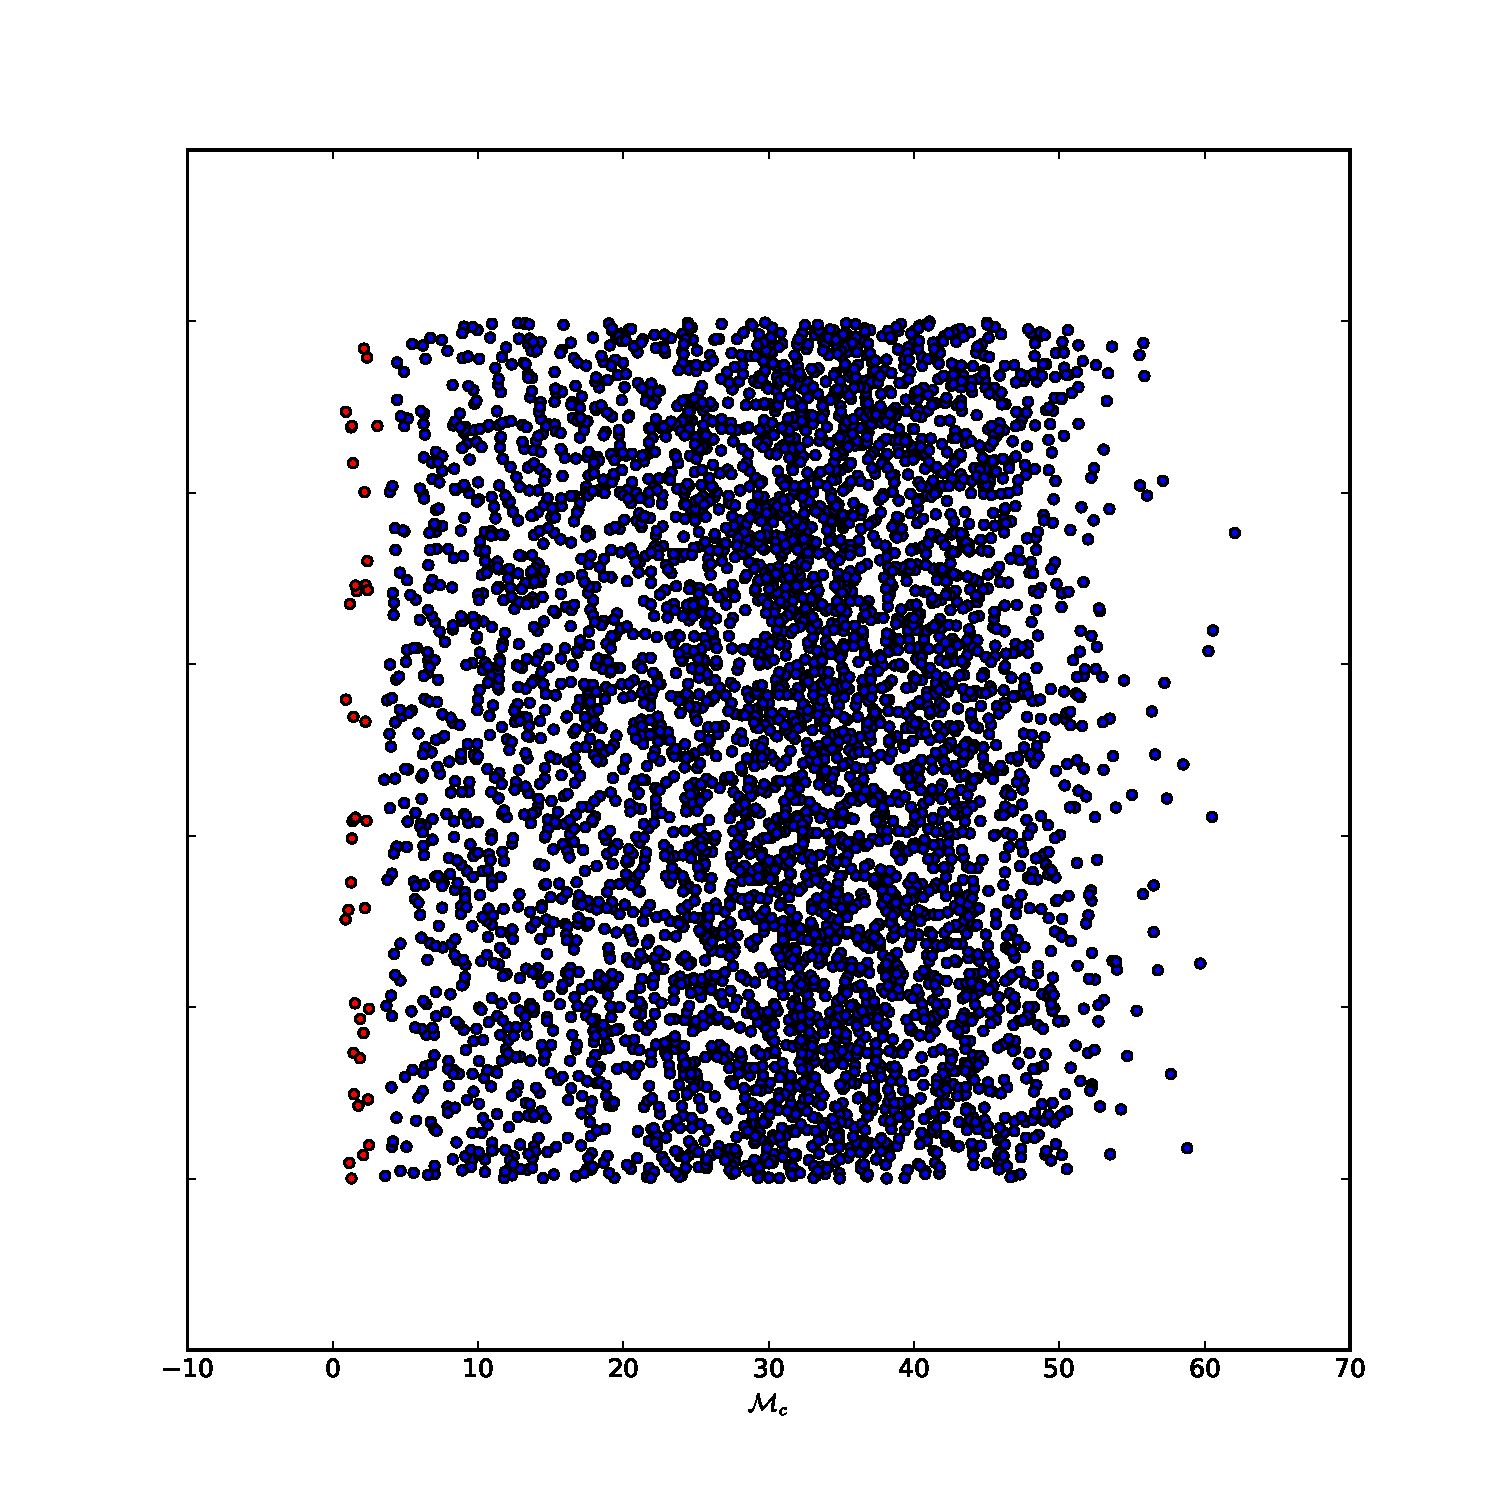
\includegraphics[width=\columnwidth]{output/jake/chirp-mass-classes.pdf}
\caption{This figure shows all the 5000 events' chirp mass. Here the y-axis is a uniform random number between zero and one. The events that have an electromagnetic counterpart are in red, and the events without a electromagnetic counterpart are in blue.}
\label{fig:chirp}
\end{figure}
See Section \ref{sec:discussion} and Appendix \ref{app:example}. Example text citation is \textcite{2012ApJ...759...52D}, or in parenthesis with a page number \parencite[pg 2]{2012ApJ...759...52D}.

